% -*- coding: utf-8 -*-
\documentclass[UTF8,a4paper,10pt]{ctexart}
\usepackage[left=3.17cm, right=3.17cm, top=2.74cm, bottom=2.74cm]{geometry}
\usepackage{amsmath}
\usepackage{graphicx,subfig}

\usepackage{threeparttable}
\usepackage{float}
\usepackage{cite}
\usepackage{caption}
\usepackage{enumerate}
\usepackage{booktabs} %表格
\usepackage{multirow}

\newcommand{\tabincell}[2]{\begin{tabular}{@{}#1@{}}#2\end{tabular}}  %表格强制换行
%-------------------------字体设置--------------
\usepackage{ctex}
\newcommand{\yihao}{\fontsize{26pt}{36pt}\selectfont}           % 一号, 1.4 倍行距
\newcommand{\erhao}{\fontsize{22pt}{28pt}\selectfont}          % 二号, 1.25倍行距
\newcommand{\xiaoer}{\fontsize{18pt}{18pt}\selectfont}          % 小二, 单倍行距
\newcommand{\sanhao}{\fontsize{16pt}{24pt}\selectfont}  %三号字
\newcommand{\xiaosan}{\fontsize{15pt}{22pt}\selectfont}        % 小三, 1.5倍行距
\newcommand{\sihao}{\fontsize{14pt}{21pt}\selectfont}            % 四号, 1.5 倍行距
\newcommand{\banxiaosi}{\fontsize{13pt}{19.5pt}\selectfont}    % 半小四, 1.5倍行距
\newcommand{\xiaosi}{\fontsize{12pt}{18pt}\selectfont}            % 小四, 1.5倍行距
\newcommand{\dawuhao}{\fontsize{11pt}{11pt}\selectfont}       % 大五号, 单倍行距
\newcommand{\wuhao}{\fontsize{10.5pt}{15.75pt}\selectfont}    % 五号, 单倍行距
%-------------------------章节名----------------
\usepackage{ctexcap}
\CTEXsetup[name={,、},number={ \chinese{section}}]{section}
\CTEXsetup[name={（,）},number={\chinese{subsection}}]{subsection}
\CTEXsetup[name={,.},number={\arabic{subsubsection}}]{subsubsection}
%-------------------------页眉页脚--------------
\usepackage{fancyhdr}
\pagestyle{fancy}
\lhead{\kaishu \leftmark}
\rhead{\kaishu 自然语言处理作业报告}
\lfoot{}
\cfoot{\thepage}
\rfoot{}
\renewcommand{\headrulewidth}{0.1pt}
\renewcommand{\footrulewidth}{0pt}%去掉横线
\newcommand{\HRule}{\rule{\linewidth}{0.5mm}}%标题横线
\newcommand{\HRulegrossa}{\rule{\linewidth}{1.2mm}}
%-------------------------代码-------------------
\usepackage{xcolor}
\usepackage{listings}
\lstset{
breaklines,%自动换行
basicstyle=\small,
escapeinside=``,
keywordstyle=\color{ blue!70} \bfseries,
commentstyle=\color{red!50!green!50!blue!50},%
stringstyle=\ttfamily,%
extendedchars=false,%
linewidth=\textwidth,%
numbers=left,%
numberstyle=\tiny \color{blue!50},%
frame=trbl%
rulesepcolor= \color{ red!20!green!20!blue!20}
}
%------------超链接----------
\usepackage[colorlinks,linkcolor=black,anchorcolor=blue]{hyperref}
%------------------------TODO-------------------
\usepackage{enumitem,amssymb}
\newlist{todolist}{itemize}{2}
\setlist[todolist]{label=$\square$}
%------------------------水印-------------------
\usepackage{tikz}
\usepackage{xcolor}
\usepackage{eso-pic}

\newcommand{\watermark}[3]{\AddToShipoutPictureBG{
\parbox[b][\paperheight]{\paperwidth}{
\vfill%
\centering%
\tikz[remember picture, overlay]%
  \node [rotate = #1, scale = #2] at (current page.center)%
    {\textcolor{gray!80!cyan!30!magenta!30}{#3}};
\vfill}}}

\graphicspath{{figures/}}

%====================================================正文=====================================================
\begin{document}
\begin{titlepage}
    \begin{center}
    
\includegraphics[width=0.8\textwidth]{NKU.png}\\[1cm]
    \textsc{\Huge \kaishu{\textbf{南\ \ \ \ \ \ 开\ \ \ \ \ \ 大\ \ \ \ \ \ 学}} }\\[0.9cm]
    \textsc{\huge \kaishu{\textbf{计\ \ 算\ \ 机\ \ 学\ \ 院}}}\\[0.5cm]
    \textsc{\Large \textbf{自然语言处理作业报告}}\\[0.8cm]
    \HRule \\[0.9cm]
    { \LARGE \bfseries 新闻文本分类：从词袋到 BERT}\\[0.4cm]
    \HRule \\[2.0cm]
    \centering
    \textsc{\LARGE 邹博闻\kaishu{\ \ \ \ }}\\[0.5cm]
    \textsc{\LARGE \kaishu{年级\ :\ 2023级}}\\[0.5cm]
    \textsc{\LARGE \kaishu{专业\ :\ 计算机科学与技术}}\\[0.5cm]
    \textsc{\LARGE \kaishu{学号\ :\ 2312251}}\\[0.5cm]
    \vfill
    {\Large \today}
    \end{center}
\end{titlepage}
%----------------------------------------------------------------
\tableofcontents
%----------------------------------------------------------------
\newpage
\watermark{60}{10}{NKU}
\setcounter{page}{1}

\section{任务描述}

本次作业的目标是在 NYT 数据集上做新闻文本分类，把每篇文章分到 business、politics、sports 三个类别之一。数据分成了训练、验证、测试三份，比例为 8:1:1。评测指标是 Accuracy 和 Macro F1。

任务要求按三个步骤递进完成，每步用不同的文本表示方法做同一个分类任务：

（1）\textbf{T1}：Bag-of-Words + 逻辑回归（Logistic Regression）。特征有两种做法，一是 binary bag，只记录词是否出现；二是 word frequency，记录词出现的频数。

（2）\textbf{T2}：word2vec 词向量。先在无标签文本上训练词向量，把文档表示成词向量的某种聚合，再训练分类器。

（3）\textbf{T3}：BERT。用预训练的 BERT 模型做微调（fine-tune）完成分类。

笔者的做法是三条路径全部实现：T1 除二值词袋外补了 TF-IDF 变体，T2 按作业要求做了预训练 GloVe、AG News 自训 word2vec、NYT 自训 word2vec 三组实验，T3 除全量微调外补了冻结 encoder 的线性探测作对照。T3 使用了服务器上的 Ascend 950 NPU 加速训练，过程中还踩到一个 torch\_npu 的坑，后面单独说。

\section{数据集分析}
\subsection{基础分析}

数据给了两个 csv 文件：

\begin{lstlisting}[frame=single,numbers=none]
nyt.csv : text, label     （有标签，用于分类）
ag.csv  : text            （无标签，9 万条 AG News 文本）
\end{lstlisting}

nyt.csv 是任务指定的分类数据集。ag.csv 没有标签，笔者的判断是它作为 T2 无监督训练 word2vec 的语料，9 万条新闻文本量足够训练词向量，而 NYT 自己只有一万多篇，直接拿来训词向量词表会很稀疏。这个判断在后面的实验里得到了验证：用 ag.csv 训出的词向量在 NYT 测试集上的词表覆盖率达到 95.9\%。

\subsection{数据统计}

两个文件的基本统计如下。

\begin{table}[h]
\centering
\caption{数据集基本统计}
\label{tab:data_stat}
\begin{tabular}{|c|c|c|}
\hline
\textbf{指标} & \textbf{nyt.csv} & \textbf{ag.csv} \\ \hline
样本数 & 11,519 & 90,000 \\ \hline
列 & text, label & text \\ \hline
类别数 & 3 & 无标签 \\ \hline
\textbf{sports} & 8,639（75.0\%） & 无 \\ \hline
\textbf{politics} & 1,451（12.6\%） & 无 \\ \hline
\textbf{business} & 1,429（12.4\%） & 无 \\ \hline
\end{tabular}
\end{table}

从数字里能看出两个需要注意的点：

（1）\textbf{类别严重不均衡}。sports 占了四分之三，politics 和 business 加起来才四分之一。如果只报 Accuracy，一个全猜 sports 的模型也能有 75\%，所以报告里同时给出 Macro F1，它把三个类别同等看待，能反映少数类的表现。

（2）\textbf{文本都很长}。NYT 的文章大多有几百词，T3 用 BERT 时受序列长度限制必须截断，这会损失一部分上下文信息，后面实验结果里会看到它对准确率的影响。

\section{T1：Bag-of-Words + 逻辑回归}

\subsection{方法}

T1 的做法很直接：先把每篇文档用一个向量表示，向量的每一维对应词表里的一个词，然后训练逻辑回归分类。

binary bag 和 word frequency 的区别只在向量的取值上：

$$v_i = \begin{cases}
\mathbb{I}[\text{词 } i \text{ 出现在文档中}] & \text{binary bag}\\
\text{count}(i) & \text{word frequency}
\end{cases}$$

这里 count$(i)$ 是词 $i$ 在文档里出现的次数。两个版本都去了英文停用词，词表上限 5 万。逻辑回归的惩罚系数 $C$ 在验证集上网格搜索（0.1、0.5、1、5、10），取验证 Accuracy 最高的一组，最后在测试集上报数。

\textbf{加分项：TF-IDF。} TF-IDF 是词袋家族里最常见的升级：词频再乘一个逆文档频率，压制那些到处都是、没什么区分度的词：

$$\text{tfidf}(i) = \text{count}(i) \cdot \log\frac{N}{\text{df}(i)}$$

$N$ 是文档总数，$\text{df}(i)$ 是出现过词 $i$ 的文档数。把它加进来，是想看看"词袋还能不能再压一点分"。

\subsection{实验结果}

\begin{table}[htbp]
\centering
\caption{T1 测试集结果}
\label{tab:t1}
\begin{tabular}{cccc}
\toprule
\textbf{变体} & \textbf{特征含义} & \textbf{Accuracy} & \textbf{Macro F1} \\
\midrule
(1) binary bag & 词是否出现（0/1） & 0.9913 & 0.9778 \\
(2) word frequency & 词频计数 & 0.9931 & 0.9834 \\
(3) TF-IDF（加分） & 词频 $\times$ IDF & \textbf{0.9939} & \textbf{0.9857} \\
\bottomrule
\end{tabular}
\end{table}

三个变体都到了 0.99 以上，词袋在这个任务上确实很强。从 binary 到 word frequency，多了"出现几次"的信息，Macro F1 涨了 0.56 个百分点；到 TF-IDF 又小幅上涨。差异不算大，但方向一致：词频比二值更丰富，IDF 又比纯词频更能压住高频虚词。

\subsection{各类别判别词}

逻辑回归的系数可以直接解释：每个类别系数最高的那批词，就是模型认为最能代表这个类的语言特征。

\begin{lstlisting}[frame=single,numbers=none]
business: company, market, percent, industry, billion, bank, trade ...
politics : mr, washington, republican, obama, senator, house, texas ...
sports   : players, league, game, team, football, tournament, coach ...
\end{lstlisting}

词和类别的对应很干净，这也从侧面说明 NYT 新闻的主题特征是明显的，词袋模型够用。

\section{T2：Word2Vec 词向量}

\subsection{三种词向量来源}

按作业要求，本部分所有词向量统一为 \textbf{100 维}，分类器统一用逻辑回归，文档表示统一用“词向量取平均”。需要完成三组实验：

（1）\textbf{预训练 GloVe}。使用公开的 \texttt{glove.6B} 中的 100 维词向量 \texttt{glove.6B.100d.txt}（共 40 万词）。这是在大规模通用语料上预训练好的词表示，本任务直接查表使用。

（2）\textbf{在 AG News 上训练 word2vec}。用 9 万条无标签的 ag.csv 文本训练一个 100 维 skip-gram 模型（窗口 5，min\_count=5 丢弃低频词，训练 5 轮）。这是作业指定的做法，借用外部新闻语料缓解 NYT 自身语料偏小的问题。

（3）\textbf{在 NYT 上训练 word2vec}。用 NYT 自身的文本（训练集部分）训练同样配置的 100 维 skip-gram 模型，与（2）形成对照，看外部语料是否有帮助。

word2vec 两次训练分别只花了约 19 秒（AG，词表 22,504）和 34 秒（NYT，词表 27,051）。

\subsection{文档表示}

对一篇包含 $n$ 个有效词（即在词表中出现的词）的文档，取其所有词向量的平均作为文档向量：

$$\vec{d} = \frac{1}{n}\sum_{i=1}^{n} \vec{w}_i$$

再把得到的 100 维文档向量送入逻辑回归分类，惩罚系数 $C$ 在验证集上网格搜索（0.1、0.5、1、5、10），最后在测试集上报数。

\subsection{实验结果}

\begin{table}[htbp]
\centering
\caption{T2 测试集结果（100 维词向量 + 均值文档表示）}
\label{tab:t2}
\begin{tabular}{cccc}
\toprule
\textbf{词向量来源} & \textbf{维度} & \textbf{Accuracy} & \textbf{Macro F1} \\
\midrule
(1) 预训练 GloVe（glove.6B） & 100 & 0.9861 & 0.9669 \\
(2) word2vec 训练于 AG News & 100 & 0.9844 & 0.9613 \\
(3) word2vec 训练于 NYT & 100 & \textbf{0.9887} & \textbf{0.9727} \\
\midrule
T1 词频 BoW（参照） & 50,000 & 0.9931 & 0.9834 \\
\bottomrule
\end{tabular}
\end{table}

三组结果都在 0.98 以上，彼此差距不到半个百分点，比 T1 词袋低了约 0.5$\sim$1 个百分点。原因不难理解：把整篇文章压成一个 100 维稠密向量，均值池化本身丢掉了大量信息，而词袋虽然稀疏高维，但保留的信息更完整。两个观察值得记录：

（1）\textbf{预训练 GloVe 与自训练 word2vec 基本打平}。GloVe 在通用大语料上训练，词表覆盖率高（NYT 测试集有效词覆盖率 99.8\%），但和用 9 万条 AG News 现训的模型（覆盖率 95.9\%）分数几乎一样（0.9861 对 0.9844）。说明新闻主题分类对词级语义的要求不高，通用词向量与领域词向量差别不大。

（2）\textbf{NYT 自训反而最好}。用 NYT 自身训练的 word2vec 取得最高的 0.9887/0.9727，比 AG 版高约 0.4 个百分点，推测是领域与任务更贴合。不过三组差距很小，说明这条稠密表示路线上，词向量的来源不是主要瓶颈。

\subsection{词向量语义验证}

虽然分类分数不如词袋，但词向量本身是有效的，几个直观证据（以 NYT 自训模型为例）：

\begin{itemize}
\item $\text{sim}(\text{juventus}, \text{soccer}) = 0.488$，而 $\text{sim}(\text{juventus}, \text{business}) = 0.234$，语义相近的词相似度明显更高；
\item 最近邻都是同类词：juventus $\to$ ajax, wolfsburg, fiorentina；bank $\to$ deutsche, monetary, jpmorgan；
\item 测试集词表覆盖率：预训练 GloVe 99.8\%、AG 版 95.9\%、NYT 版 98.6\%，都能覆盖绝大多数词。
\end{itemize}

把 NYT 测试集文档的均值向量用 t-SNE 降到二维，三类基本能分开，见下图。

\begin{figure}[H]
\centering
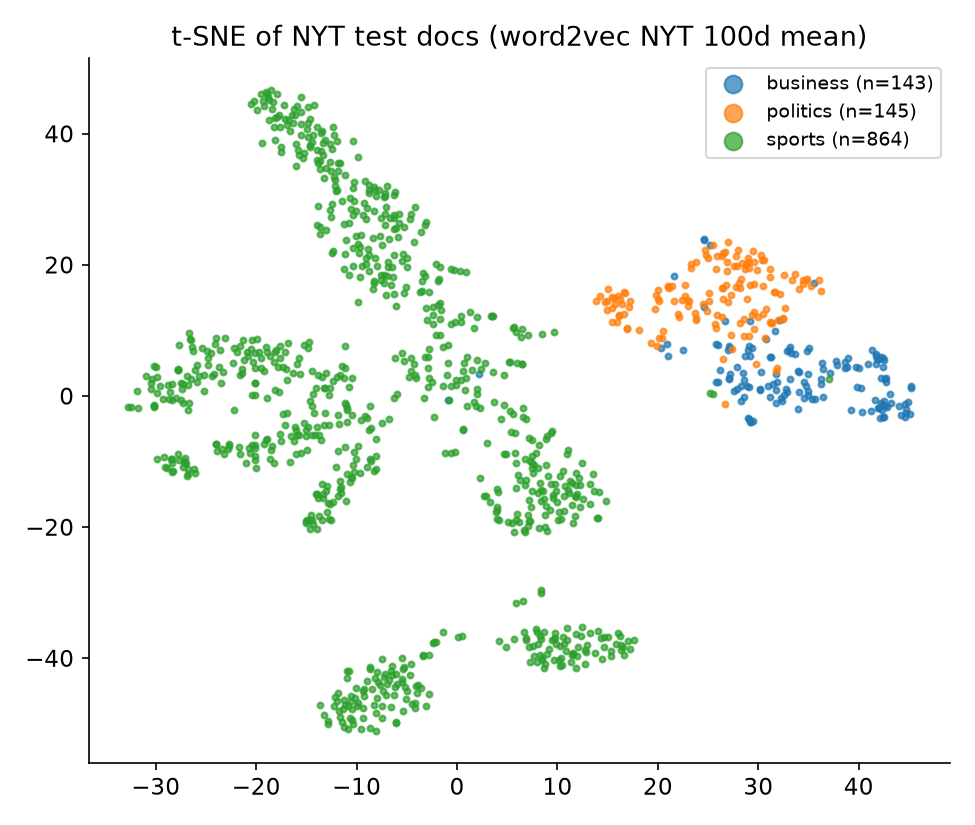
\includegraphics[width=0.6\textwidth]{fig_t2_tsne.png}
\caption{NYT 测试集文档的 t-SNE 可视化（NYT 自训 word2vec 100 维均值向量）}
\label{fig:tsne}
\end{figure}

\section{T3：BERT 微调（Ascend 950 NPU）}

\subsection{方法}

T3 用 bert-base-uncased 做序列分类微调。处理方式：按作业要求把文本截断到 64 token，损失用交叉熵并按类别加权（少数类权重更高），优化器 AdamW，学习率 $2\times10^{-5}$ 加线性 warmup，每步做梯度裁剪。训练 3 个 epoch，每个 epoch 在验证集上评一次，保留验证 Macro F1 最高的一组权重，最后在测试集上报数。

训练在服务器的 Ascend 950 NPU 上进行。这台机器配了 torch\_npu 2.10.0 + CANN 9.1.0，NPU 上 3 个 epoch 一共只用了约 1 分钟（21$\sim$23 秒/epoch）。同样的配置在 CPU 上跑，40 分钟连一个 epoch 都没跑完，NPU 大概快了 60 倍，这个加速对后续迭代调参非常有价值。

\subsection{实验结果}

\begin{table}[htbp]
\centering
\caption{T3 测试集结果}
\label{tab:t3}
\begin{tabular}{cccc}
\toprule
\textbf{方法} & \textbf{Accuracy} & \textbf{Macro F1} & \textbf{每 epoch 耗时} \\
\midrule
BERT 全量微调（NPU） & \textbf{0.9826} & \textbf{0.9624} & 21 s \\
BERT 线性探测（冻结 encoder） & 0.5182 & 0.4129 & 8 s \\
\bottomrule
\end{tabular}
\end{table}

\textbf{线性探测 vs 全量微调}：只冻结 encoder、训练分类头（线性探测）的准确率只有 0.5182，全量微调到了 0.9826。差距 0.46，是本次作业里最大的。这说明预训练 BERT 的特征虽然好，但如果不针对下游任务微调，直接用出来并不适合分类；微调才是发挥 BERT 价值的关键一步。

三个类别的 Macro F1 分别如下：sports 0.9948、business 0.9488、politics 0.9437。sports 类几乎全对，少数类要差一些，混淆矩阵见图 \ref{fig:t3cm}，学习曲线见图 \ref{fig:t3curve}。

\begin{figure}[H]
\centering
\subfloat[学习曲线]{
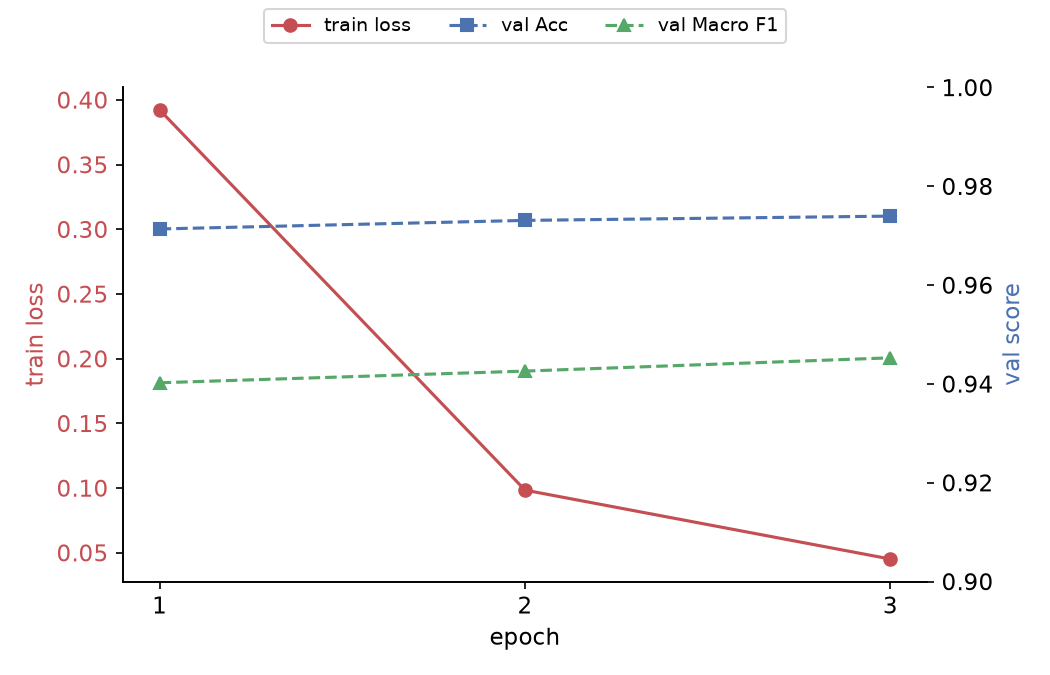
\includegraphics[width=0.48\textwidth]{fig_t3_curve.png}
\label{fig:t3curve}}
\hfill
\subfloat[混淆矩阵]{
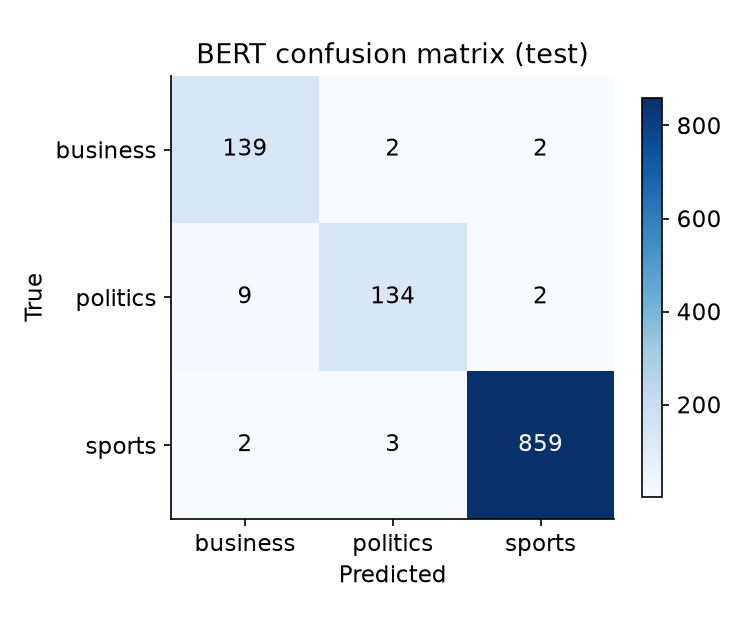
\includegraphics[width=0.42\textwidth]{fig_t3_cm.png}
\label{fig:t3cm}}
\caption{BERT 微调的学习曲线与测试集混淆矩阵}
\end{figure}

\subsection{踩坑记录：torch\_npu 在 950 上的梯度溢出}

T3 一开始并不顺利。首次在 NPU 上微调，训练到第 20 到 40 步左右 loss 突然变成 nan，验证准确率瞬间掉到随机水平。笔者花了不少时间定位，过程记录如下：

（1）先排除优化器和 dtype。AdamW、SGD、fp32、fp16、bf16 组合都试过，全部在若干步后炸，说明不是优化器的问题，也不是精度不够的问题。

（2）再排除数据。同一份数据在 CPU 上训练完全正常，锁定是 torch\_npu 在 950 上的反向传播不稳定。

（3）定位到具体参数。在梯度第一次出现 inf 的那一步打断点，发现问题出在 encoder 内部，冻结整个 encoder 只训分类头时，150 步稳定不炸。

（4）最后确定触发条件。反复测试后发现，序列长度是关键：\texttt{max\_len=128} 时训练完全稳定，\texttt{max\_len=256} 时必炸（重复实验 4 次全挂），192 和 224 也会在训练中途随机炸掉。判断是长序列上某个算子的反向梯度累加溢出。作业要求的 \texttt{max\_len=64} 远低于这个阈值，训练全程无 nan，因此最终结果采用 64。

规避办法很简单：控制序列长度（本例按作业要求取 64）并加一层梯度裁剪兜底，最终训练全程无 nan。代价是 BERT 只能看每篇文档的前 64 个 token，上下文截断损失了一点准确率。这属于 950（3510 架构）上 torch\_npu 算子兼容性问题的一例。

\section{实验结果对比}

\subsection{总对比}

把三条路径的所有结果放到一张表里：

\begin{table}[htbp]
\centering
\caption{全部方法测试集结果对比}
\label{tab:overall}
\begin{tabular}{lccc}
\toprule
\textbf{方法} & \textbf{特征维度} & \textbf{Accuracy} & \textbf{Macro F1} \\
\midrule
T1 binary BoW + LR & 50,000 稀疏 & 0.9913 & 0.9778 \\
T1 TF BoW + LR & 50,000 稀疏 & 0.9931 & 0.9834 \\
T1 TF-IDF + LR & 50,000 稀疏 & \textbf{0.9939} & \textbf{0.9857} \\
\midrule
T2 GloVe 100d 均值 + LR & 100 稠密 & 0.9861 & 0.9669 \\
T2 word2vec AG 100d 均值 + LR & 100 稠密 & 0.9844 & 0.9613 \\
T2 word2vec NYT 100d 均值 + LR & 100 稠密 & 0.9887 & 0.9727 \\
\midrule
T3 BERT 微调（NPU） & 768 上下文 & 0.9826 & 0.9624 \\
T3 BERT 线性探测 & 768 & 0.5182 & 0.4129 \\
\bottomrule
\end{tabular}
\end{table}

\begin{figure}[H]
\centering
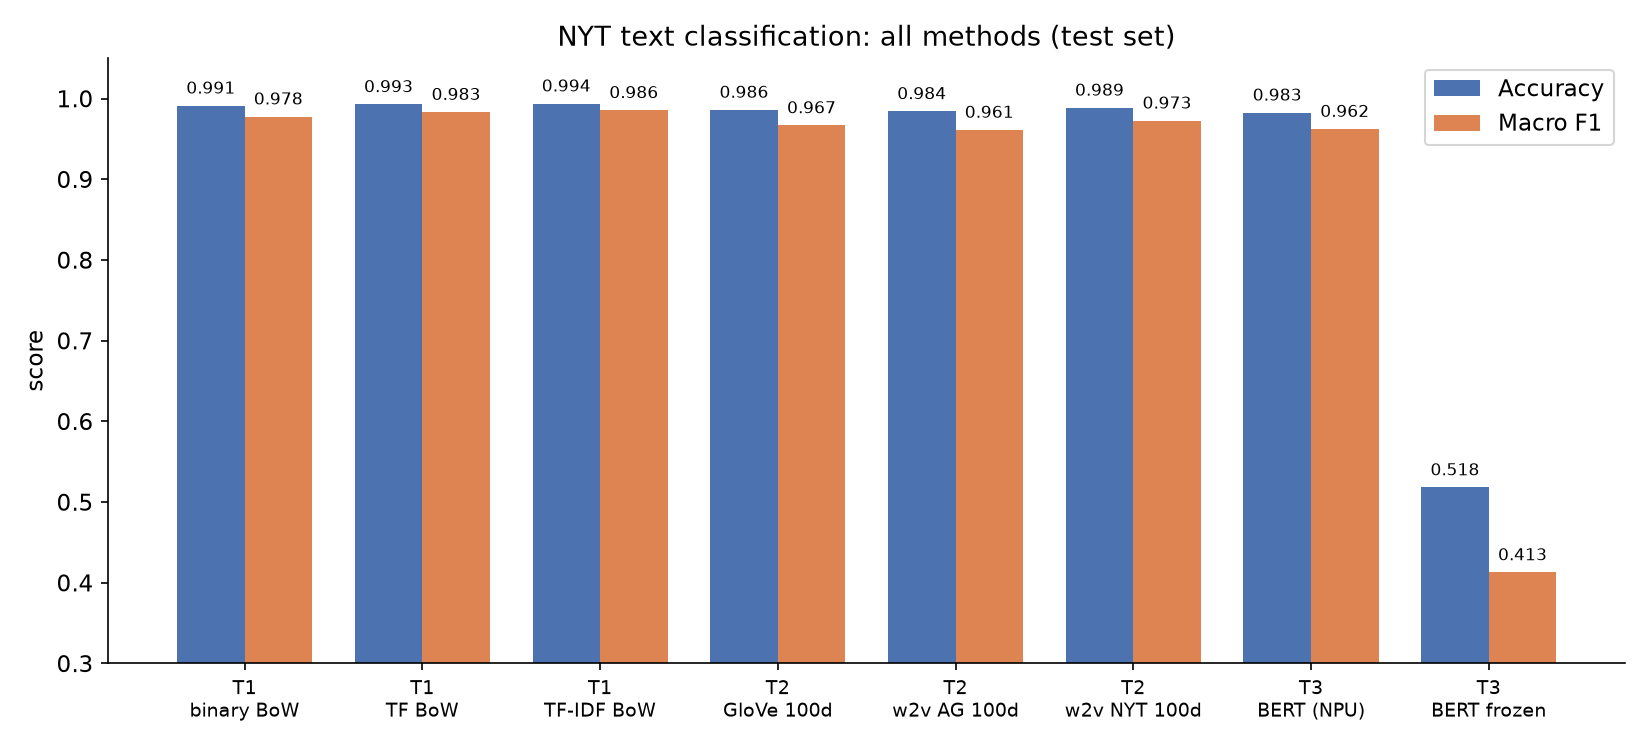
\includegraphics[width=0.72\textwidth]{fig_overall.png}
\caption{全部方法 Accuracy 与 Macro F1 对比}
\label{fig:overall}
\end{figure}

\subsection{为什么分数拉不开}

直观上看，T1 词袋（0.9939）居然比 BERT 微调（0.9826）还要高一点，有点反直觉。仔细想其实不奇怪：

（1）\textbf{任务不够难}。NYT 三个主题在词面上区分度极高，判别词实验里已经看到，business 的文章满篇是 company、market、billion，politics 满篇是 obama、senator、washington。这样的任务词袋模型已经接近上限，留给"更聪明"的模型的提升空间几乎没有了。

（2）\textbf{BERT 被截断拖累}。按作业要求 BERT 只能看 64 个 token，而词袋能看整篇文章。如果放宽序列长度，BERT 还有上升空间，但一方面受 950 上长序列反向溢出的约束，另一方面作业也指定了 64，只能接受。

（3）\textbf{T2 的均值和 BERT 的池化都丢信息}。这两条"稠密表示"路线天然比不过"看全文的词袋"，这不是方法的问题，是新闻主题分类本身对顺序和上下文不敏感。

（4）\textbf{真正的区分度在冻结 vs 微调}。全场差距最大的不是方法之间，而是 BERT 自己内部：冻结 encoder 只有 0.5182，微调后 0.9826。语义表示的价值需要下游微调来兑现。

换个角度看，三档方法对应的其实是三条技术路线：词袋的稀疏高维、词向量的紧凑低维、BERT 的上下文感知。它们的分数都在 0.97 到 0.99 之间，说明这个数据集上三档方法都"够用"了，差异主要体现在特征维度的数量级和训练开销上，而不是最终分数。

\section{总结}

本次作业把三类文本表示方法完整走了一遍，全部在同一个 8:1:1 划分上评测，保证可比。几个可以记下来的结论：

（1）词袋 + 逻辑回归是最朴素也最稳的基线，三个变体都到 0.99，TF-IDF 略优于词频、词频略优于二值。

（2）word2vec 把 5 万维的稀疏表示压缩成 100 维稠密表示，损失约一个百分点，且天然处理 OOV；预训练 GloVe、AG 自训、NYT 自训三种来源分数接近，均值文档表示就已够用。

（3）BERT 在 NPU 上微调达到 0.9826，训练只需约 1 分钟；冻结 encoder 的线性探测只有 0.5182，充分说明微调的必要性。

（4）Ascend 950 的 torch\_npu 存在长序列反向梯度溢出的问题，用受控序列长度（本例 64）+ 梯度裁剪规避。

代码、模型和图片都已放在服务器 \texttt{~/nlp/HW-1/} 目录下。本作业的完整代码与报告仓库：

\begin{center}
\url{https://github.com/QunLi123/nlp-hw1}
\end{center}

\end{document}